\documentclass[11pt,twoside]{article}

\usepackage{amsmath}
\usepackage{graphicx,epstopdf,epsfig}
\usepackage{amsmath,amssymb,amsbsy,bm}
%\usepackage[framed]{mcode}

\newlength{\toppush}
\setlength{\toppush}{2\headheight}
\addtolength{\toppush}{\headsep}

\renewcommand{\bottomfraction}{0.95}

\newcommand{\htitle}[3]{\begin{center}
\vspace*{-\toppush}
{\large MASSACHUSETTS INSTITUTE OF TECHNOLOGY}\\
{\small Department of Electrical Engineering and Computer Science}\\
\vspace*{1ex}{\Large #2}\end{center}
\noindent
\newline\parbox{6.5in}
{Fall 2013\hfill Issued : #1 \newline
 Problem Set 8 \hfill Due : #3\newline
%\profs \hfill %Handout #1\vspace*{-.5ex}\newline
%\mbox{}\hrulefill\mbox{}
}}

\newcommand{\mcO}{\mathcal{O}}
\newcommand{\handout}[3]{\thispagestyle{empty}
\pagestyle{myheadings}\htitle{#1}{#2}{#3}}

\setlength{\oddsidemargin}{0pt}
\setlength{\evensidemargin}{0pt}
\setlength{\textwidth}{6.5in}
\setlength{\topmargin}{0in}
\setlength{\textheight}{8.5in}


\newcommand{\pp}[2]{\frac{\partial #1}{\partial #2}}%
\newcommand{\ppp}[2]{\frac{\partial^2 #1}{\partial #2^2}}%
\newcommand{\dd}[2]{\frac{d #1}{d #2}}%
\newcommand{\ddd}[2]{\frac{d^2 #1}{d #2^2}}%
\newcommand{\matend}{\end{array}\right]}
\newcommand{\matc}{\left[\begin{array}{c}}
\newcommand{\matcc}{\left[\begin{array}{cc}}
\newcommand{\bb}{\mathbf{b}}
\newcommand{\bx}{\mathbf{x}}
\newcommand{\bA}{\mathbf{A}}
\newcommand{\DD}[2]{\frac{D #1}{D #2}}%
\newcommand{\Uvec}{\mathbf{U}}
\newcommand{\uvec}{\mathbf{u}}
\newcommand{\tauvec}{\bm{\tau}}
\newcommand{\omegavec}{\bm{\omega}}


\renewcommand{\Re}{\mathrm{Re}}


\begin{document}


\handout{Nov 19, 2013}{6.301 Solid State Circuits}{Nov 26, 2013}
\setlength{\parindent}{0pt}

\newcommand{\solution}{
 \medskip
 {\bf Solution:}
}

\hrulefill

\flushleft

\subsection*{Problem 1: Translinear Jungle Gym}
For each of the following circuits use the “Gilbert Principle”
to determine $I_o$ as a function of the other circuit variables.
All of these circuits simplify to simple expressions. \\
A differential output is denoted by an $I_o$ superimposed on an arrow,
 and double emitter arrows with $2A_E$ indicate that transistor has double the emitter area of the other transistors, thus its $I_S$ is twice as large. \\
Finally, use the method of open circuit time constants to estimate the $-3dB$ frequency for the circuit in part (a) only.
\vspace{8ex}
\begin{center}
\includegraphics[width=.9\textwidth]{trans1.eps}
\end{center}

\clearpage
\begin{center}
\includegraphics[width=.6\textwidth]{trans2.eps}
\end{center}
\clearpage
\subsection*{Problem 2: Translinear Approximator}
Find $I_o=f(I_x)$, assuming well-matched transistors, negligible base currents, and $I_1=1A$.
Also assume $Q_A$ and $Q_B$ have emitter areas $24A_E$ and $2A_E$, respectively, while all other transistors have emitter area $A_E$. \\
What famous function does $I_o$ approximate for small $I_x$?\\
\vspace{4ex}
\begin{center}
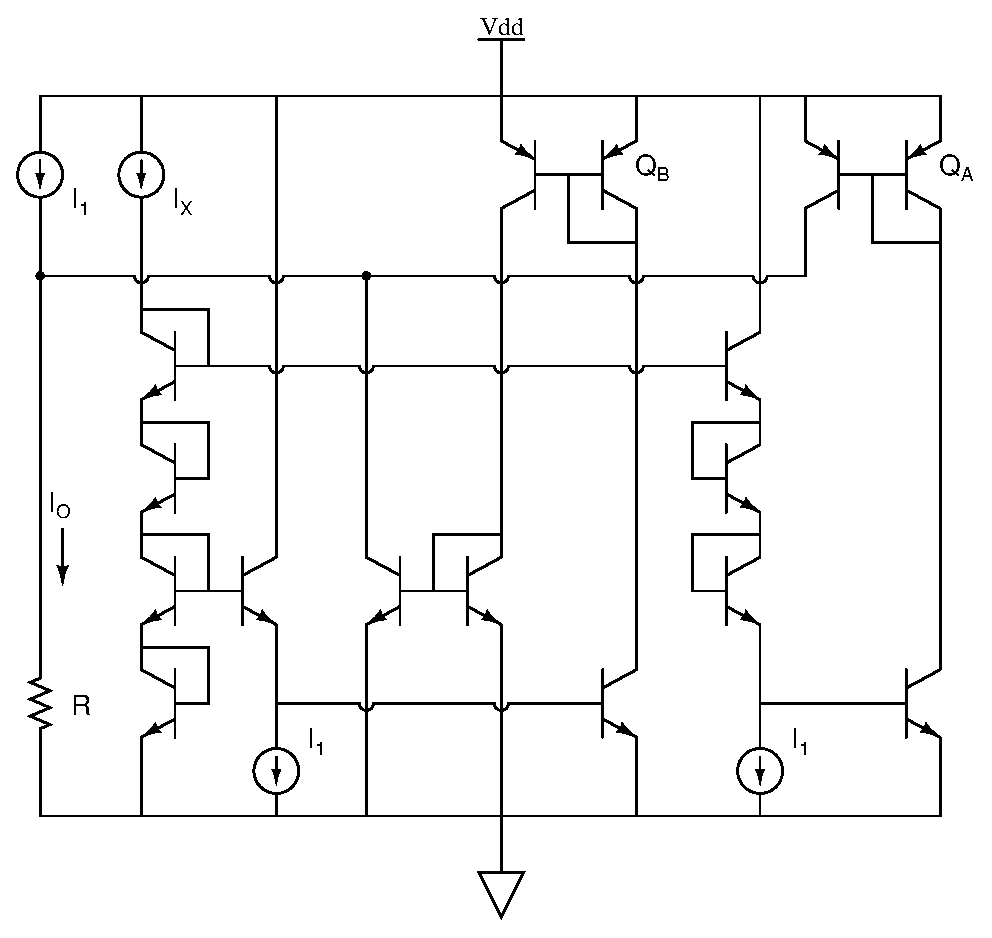
\includegraphics[width=.9\textwidth]{cos.eps}
\end{center}

\clearpage

\subsection*{Problem 3: Base Current Effects}
In the following circuit, assume $I_2=1mA$ and $\beta=100$.\\
\vspace{1ex}

\begin{center}
\includegraphics[width=.28\textwidth]{sqrtxy.eps}
\end{center}

\begin{enumerate}
	\item[(a)] Express $I_o$ in terms of $I_1$ and $I_2$.
	\item[(b)] Assume we can tolerate a maximum $I_o$ error due to $\beta$ of 50\%.  For what range of $I_1$ is this circuit valid?
\end{enumerate}

\subsection*{Problem 4: Temperature Dependence}
When we design a circuit, we prefer that it operate over a wide range of temperature.
In the following circuit, assume that $\frac{1}{R} \frac{dR}{dT}=600ppm/^{\circ}C$ and $\frac{dV_{be}}{dT}=-2mV/^{\circ}C$. \\
\vspace{1ex}
For each of the following circuits find $\frac{dI_o}{dT}$. \\
\vspace{1ex}
Additionally, find the value of $R_E$ in terms of $I_o$ that minimizes $\frac{dI_o}{dT}$.

\begin{center}
\includegraphics[width=.25\textwidth]{temp-dep.eps}
\end{center}


\end{document}
